\begin{document}
\chapter{}
\section{Least squares}\label{ch:LS}
Assuming that $A$ is a matrix of size $m\times n$, where the rank is at least $n$, $\bf x$ a vector of parameters and $\bf b$ a vector of outputs, then the set of equations are expressed as
\begin{align}
A{\bf x}={\bf b}. \nonumber
\end{align}
If $m>n$, the equation 
\begin{equation}
A{\bf x}-{\bf b}=0 \nonumber
\end{equation}
generally doesn't have a solution. Instead, a cost function $Q$ expresses the square error of the system, defined as 
\begin{align}
Q 	&=({\bf y}-A{\bf x})^T({\bf y}-A{\bf x})\\
	&={\bf y^Ty}-2{\bf x}^TA^TA+{\bf x}A^TA{\bf x}.
\end{align}

The vector ${\bf \hat{x}}$ is the parameters which minimizes the norm of $Q$, which is expressed as
\begin{align}\label{argmin}
		{\bf \hat{x}}&=\operatorname*{argmin}_{\bf x}(||{\bf y}-A{\bf x}||). 
\end{align}
The solution to \ref{argmin} is found through finding the zeros to the derivative of $Q$ with respect to all parameters in $\bf x$, 
\begin{align*}
\frac{\partial Q}{\partial {\bf x}}&=-2A^T{\bf y}+2A^TA{\bf x}=0
\end{align*}	
which is where 
\begin{equation}
A^T{\bf y}=A^TA{\bf \bf{x}}.
\end{equation}
for some value $\bf \hat{x}$. Multiplying both sides with the inverse to $A^TA$ and thus the least square solution is given as
\begin{align}		
	{\bf \hat{x}}=(A^TA)^{-1}A^T{\bf y} \label{LS_theory}\\
\end{align}
\subsection{Weighted Least Squares}\label{ch:WLS}
This can be extended to a more general case to capture the uncertainties of the individual measurements. Assume that the matrix $W$ contains the variances of the noise and is a diagonal matrix defined as
\begin{equation}
W=\begin{bmatrix}
\sigma^2_1 &0 & \dots \\ 
0 & \sigma^2_2& 0& & \\
\vdots & & \ddots & 0 & \\
0 & \dots & 0 & \sigma^2_m
\end{bmatrix}.
\end{equation}
Then a Best Linear Unbiased Estimator (BLUE) estimation can instead be given by:
\begin{equation}
{\bf \hat{x}}_{BLUE}=(A^TWA)^{-1}A^TW{\bf y} \label{WLS_theory}
\end{equation}
The full derivation of the BLUE model can be found in \cite{moser1996linear}.

\section{Data structs and log format}\label{structsAndLogs}
The INS unit provides several possible struct types of information which can be sampled at different frequencies depending on the type, where GNSS-signals can be sampled at up to 5 Hz, while the IMU offers sampling up to 250 Hz. Among them there are both relatively unprocessed as well as processed data. A few data structs have been sampled from in this project and will be described briefly:
\begin{itemize}
\item \texttt{ins\_1\_t} - Fused data from IMU and GNSS sensors, including position (LLA/NED), velocity (body frame) and sampling time.
\item \texttt{gps\_pos\_t} - Pure GPS receiver processed data, including global position (ECEF/LLA), DOP, and sampling time.
\item \texttt{gps\_raw\_t} - Raw observation data, including number of observations, data and data type (needed for the following fields).
\item \texttt{obsd\_t} - Raw observation data, contains receiver sampling time, satellite number, SNR (0.25dBHz), observation data carrier phase and observation pseudorange.
\item \texttt{eph\_t} - Satellite ephemeris data, contains information on satellite number, time of data transmission and time for ephemeris data issue, as well as all data mentioned in section \ref{chap:ephPositioning}.
\end{itemize}
The sampled data is saved in separate logs for each receiver for later processing. For the ephemeris log file the format is a single row for each observation including time of reception. For the observation data, the data in each epoch comes in a package of multiple observations. One whole package of observation will be logged in one row, with number of observation, time of reception shared for all followed by satellite data, SNR, loss of lock indicator, code indicator and observation data repeated in the following format: \\
\texttt{ \#obs, time1, time2,[satNo, SNR, LLI, code, P],[satNo, SNR, ...}\\
e.g.\\
\hspace{-2 cm}2,1562426103,0.391000,22,112,2,1,21772765.735608,41,76,0,1,20961030.484006,

\section{Global position and onboard estimates}
The position estimates from the onboard and global position estimator are shown together for the two sampling series in figure \ref{fig:onboardAndGlobal}.

\begin{figure}[H]
\begin{subfigure}{1.2\textwidth}
\includegraphics[width=1\textwidth]{Appendix/GlobalPosAndGPSNorth}
\subcaption{Position estimate in a NED-frame for separated by a 10 m baseline in a north direction.}
\end{subfigure}
\begin{subfigure}{1.2\textwidth}
\includegraphics[width=1\textwidth]{Appendix/GlobalPosAndGPSEast}
\subcaption{Position estimate in a NED-frame for separated by a 10 m baseline in an east direction.}
\end{subfigure}
\caption{\label{fig:onboardAndGlobal} Independent global position estimates for two receivers separated 10m N-direction (upper) and E-direction (lower), origin is set to true position. The onboard estimate is plotted together with the global position estimator.}
\end{figure}

\begin{figure}[!htb]
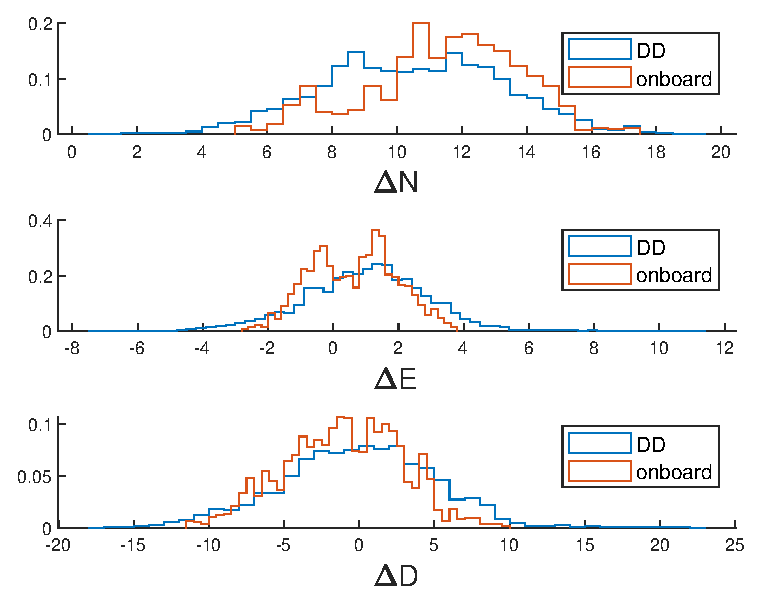
\includegraphics[width=\textwidth]{Results/Nhist.eps}
\caption{\label{fig:DDandInternalN} Histogram over difference in position over time with a North direction baseline of 10 m. Plots showing results of DD and onboard solution.}
\end{figure}
\begin{figure}[!htb]
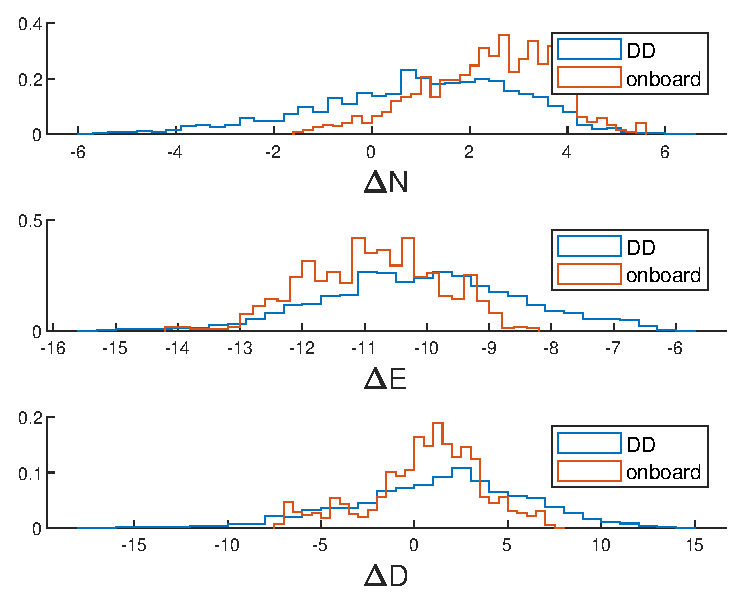
\includegraphics[width=\textwidth]{Results/Ehist.eps}
\caption{\label{fig:DDandInternalE} Histogram over difference in position over time with an East direction baseline of 10 m. Plots showing results of DD and onboard solution.}
\end{figure}

\end{document}